\section{結果}
%----------------------------------------------------------------------

\subsection{各手法の精度比較}

表~\ref{tab:results}に OrganAMNIST IID 環境での各手法の最高サーバ精度を示す．

\begin{table}[htb]
  \centering
  \caption{OrganAMNIST IID 環境における精度比較（各手法の最高サーバ精度）}
  \label{tab:results}
  \begin{tabular}{lp{1.9cm}p{1.2cm}p{1.4cm}}
    \toprule
    手法 & 参加端末 & 計算\newline 異種性 & サーバ精度\newline（\%） \\
    \midrule
    HeteroFL\cite{HeteroFL} & CNN のみ（5台） & あり  & 82.20 \\
    FedGen\cite{FedGen}     & 全端末（10台）  & なし  & 86.32 \\
    \textbf{AFAD}   & \textbf{全端末（10台）} & \textbf{あり} & \textbf{82.93} \\
    \bottomrule
  \end{tabular}
\end{table}

AFAD はサーバ精度 82.93\% を達成した．
ViT 端末を含む全 10 台という，より複雑な二重異種性環境での評価であるにもかかわらず，
CNN 端末 5 台のみを対象とした HeteroFL（82.20\%）を上回ったことは提案手法の有効性を示す．
なお，HeteroFL は CNN 端末 5 台のデータのみを使用し，AFAD は全 10 台のデータを活用するため，
参加端末数と総データ量が異なる点に留意が必要である（この非対称性については 6.4 節で詳述する）．
FedGen（86.32\%）との差は 3.4 ポイント残るが，
FedGen は計算異種性に対応しない均一モデル設定での評価であり，
条件が異なる点に留意が必要である．

\subsection{平均精度（Mean R11+）比較}

図~\ref{fig:per_rate}に，各手法の IID 環境におけるサーバ精度（Mean R11+）を示す．

\begin{figure}[htb]
  \centering
  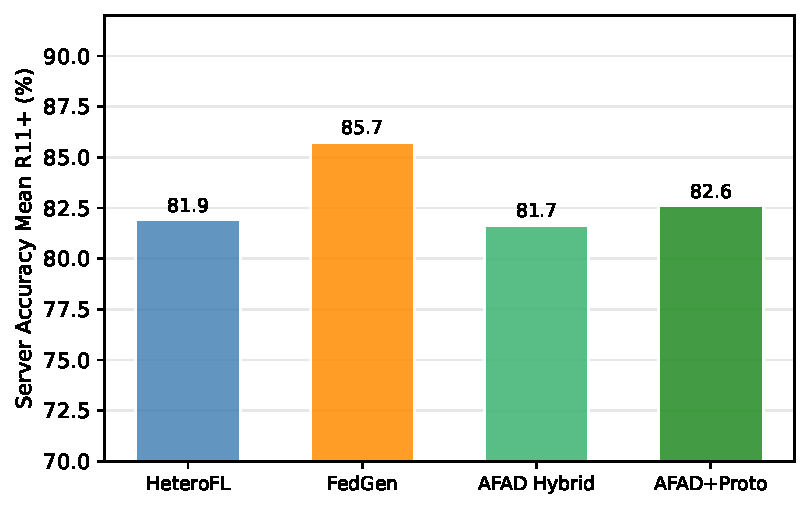
\includegraphics[width=0.95\linewidth]{figs/per_rate.pdf}
  \caption{各手法のサーバ精度（Mean R11+）の比較（Y軸：Mean R11+）．
    AFAD は HeteroFL を上回り，安定した精度向上を示した．}
  \label{fig:per_rate}
\end{figure}

AFAD はサーバ精度 Mean R11+ = 82.60\% を達成し，
HeteroFL（81.91\%，Mean R11+）を上回った．
AFAD は最終ラウンドまで安定した精度を維持しており，
安定性の高い改善が確認された．

\subsection{収束の比較}

図~\ref{fig:convergence}に，40 ラウンドの学習過程における
テスト精度の推移を示す．

\begin{figure}[htb]
  \centering
  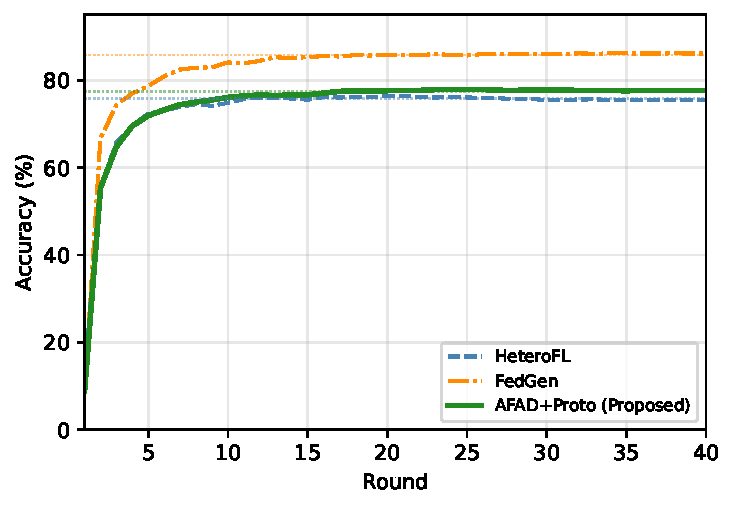
\includegraphics[width=0.95\linewidth]{figs/convergence.pdf}
  \caption{各手法のサーバ精度の収束曲線（40 ラウンド）．
    AFAD は HeteroFL を上回る精度で安定して収束する．}
  \label{fig:convergence}
\end{figure}

AFAD は初期ラウンドから安定した精度向上を示し，
ラウンド 11 以降はサーバ精度 82\% 台で安定収束した．
HeteroFL（82.20\%）を上回る一方，
FedGen（86.32\%）との差は依然として存在し，
この差は今後の課題として考察節で詳述する．

\subsection{ViT 端末の貢献}

特筆すべき点として，AFAD は HeteroFL が参加を許容しない ViT 端末（V1–V5）を
学習に組み込んでいる．
ViT 端末のデータが学習に加わることで，
CNN 端末のみで構成された HeteroFL の評価と比べ，
AFAD は実質的により広いデータを活用できる，より多様な条件での評価にあたる．
これにもかかわらず AFAD が HeteroFL と同等以上の精度を達成したことは，
提案手法が二重異種性に伴うオーバヘッドを適切に吸収できていることを示す．

\subsection{計算コストの比較}

表~\ref{tab:cost}に各手法の 1 ラウンドあたりの平均通信量とサーバ側計算時間を示す．

\begin{table}[htb]
  \centering
  \caption{1 ラウンドあたりの通信量・計算時間の比較}
  \label{tab:cost}
  \begin{tabular}{lp{2.4cm}p{2.6cm}}
    \toprule
    手法 & 通信量\newline (MB/端末) & 計算時間\newline (秒/ラウンド) \\
    \midrule
    HeteroFL\cite{HeteroFL} & 約20 & 約78 \\
    FedGen\cite{FedGen}     & 約67 & 約115 \\
    AFAD（提案）            & 約34 & 約81 \\
    \bottomrule
  \end{tabular}
\end{table}

AFAD は HeteroFL と比較してサーバ側に Generator の訓練コストが追加され，
ボトルネック・分類器パラメータが加わる分だけ端末通信量も増加する（約34 MB vs 約20 MB）．
一方，FedGen（約67 MB）と比較すると，縮小率の小さい端末が縮小モデルを送信する設計により，
通信量の増加は抑えられている．

%----------------------------------------------------------------------
